\documentclass[runningheads,a4paper]{llncs}

\usepackage{amssymb}
\setcounter{tocdepth}{3}
\usepackage{graphicx}
\usepackage{pifont}
\usepackage{todonotes}
\usepackage{indentfirst}

\usepackage[nomain,acronym]{glossaries}
\setacronymstyle{long-short}
\newacronym{ai}{AI}{Artificial Intelligence}
\newacronym{mcts}{MCTS}{Monte Carlo Tree Search}
\newacronym{pimc}{PIMC}{Perfect Information Monte Carlo}
\newacronym{gib}{GIB}{Ginsberg's Intelligent Bridgeplayer}
\newacronym{pipma}{PIPMA}{Perfect Information Post-Mortem Analysis}

\usepackage{url}
\urldef{\mailfc}\path|filipacorreia@tecnico.ulisboa.pt| 
\newcommand{\keywords}[1]{\par\addvspace\baselineskip
\noindent\keywordname\enspace\ignorespaces#1}

\newcommand*{\Comb}[2]{{}^{#1}C_{#2}}%

\begin{document}

\mainmatter

\title{EMYS: a social robot that plays "Sueca"}
\titlerunning{EMYS: a social robot that plays "Sueca"}
\author{Filipa Correia}
\authorrunning{EMYS: a social robot that plays "Sueca"}
\institute{Instituto Superior Técnico\\ University of Lisbon}

\maketitle


\begin{abstract} \label{abstract}

Regarding the needs of elder population, technology can be the answer to some of them.
Existing robots already guide the elderly walking through the house, or are companions for cuddling and petting. In the same way, this work aims to create a companion robot that plays the card game \emph{Sueca}. The idea is to develop an entertaining and pleasuring environment that can, additionally, stimulate their reasoning.
After reviewing the related work, this report proposes an artificial player based on Monte Carlo methods and the architecture that will use it. Considering the game state, the chosen move and some of the environment perceptions, this robot must produce an appropriate behaviour to be considered socially present during the game.


\keywords{Artificial Intelligence, Trick-taking Card Game, Hidden Information, Interactive Companions, Socially Intelligent Behaviour}
\end{abstract}
\section{Introduction} \label{introduction}

The ageing population has been increasing over the years.
As a result, some concerns about the elderly have also augmented.
Most of the time, there are special needs due to their physical disabilities.
Similarly, there is a worry about keeping them entertained, and so, it is crucial to find appropriate activities for them.
These activities may range from training their cognitive functions to just accompanying them.
Hence, all these concerns are commonly being solved with the help of technology.
For instance, there is software suitable for training memory problems due to Aphasia \cite{Pompili2011}.
Another example that can illustrate the presence of technology in the elderly lives is a robot.
Robots are already being used to remind them to take their medicine or to vacuum their floors.
However, occupying their free time with pleasuring activities continues to be a challenging task.


In parallel with the idea previously mentioned, computer programs that play games have been an interesting challenge over the years for \gls{ai}.
From board games to card games, or even role-playing games, the goal is to create rational agents capable of evaluating the game and achieving the best outcome.
Deep Blue, Chinook and Watson are good examples that have raised the bar for developing this kind of agents.
Deep Blue is a remarkable chess player and has defeated the human world champion in 1997 \cite{Campbell2002}.
Schaeffer et al. have solved Checkers with Chinook program and proved the game leads to a draw with two optimal players \cite{Schaeffer1996}.
Lastly, Watson is the \gls{qa} system that has beat the two highest ranked Jeopardy players in 2011 \cite{Ferrucci2010}.
\gls{qa} systems are so impressive due to the scope of \gls{ai} they include (i.e. natural language processing, machine learning, knowledge representation, automated reasoning, and information retrieval).
All these agents are good baselines to improve \gls{ai} in games.


Besides building programs that try to think rationally or humanly, \gls{ai} has also another branch that aims to act humanly \cite{Russell2009}.
This concern arises from the inclusion of robots in humans' life.
%Most of these robots' purpose is doing certain tasks that are currently being done by humans (i.e. vacuum the floor, play football or drive a car).
Consequently, they have to behave properly in those environments.
Considering these robots are surrounded by humans, the way they interact and communicate with people is a relevant concern.
The human-robot interaction field explores the social integration of robots with humans.


Card games are a good example of activities that aged people enjoy doing to occupy their free time.
Moreover, some of existing card games still are unsolved challenges for \gls{ai}.
Additionally, including this artificial player into an embodied agent brings \gls{hri} concerns.
As a result, the goal of this project is to integrate a social robot with aged humans in a card game scenario.
The chosen card game is \emph{Sueca}, a well known Portuguese game among the ageing population.
It is a great opportunity to relate the concerns mentioned above.
On one hand, this agent should play the game correctly.
After analysing the given hand, dealt at the beginning of the game, it should make good choices about what cards should be played.
On the other hand, this embodied agent should act accordingly to the environment of this scenario.
Since \emph{Sueca} is a four-player game with two teams, it involves an opponent and a companion role.
\todo{Desenvolver esta questao}
Every player should be engaged in the game with its verbal interaction and behaviours.



\subsection{Goals}
\label{sec:goals}

The main goals of this project are:
\begin{itemize}
\item Develop a robotic agent capable of playing and winning the \emph{Sueca} card game;
\item Include social behaviours on an embodied agent in order to act according to the game state;
\item Evaluate the correctness and advantages of the proposed system.
\end{itemize}

\subsection*{\centering*}

The next section presents some background research that helps the reader to understand the problems further mentioned (Section~\ref{sec:background}).
The report proceeds with the state-of-art of playing card-games and human-robot-interaction with the elderly (Section~\ref{sec:related-work}).
Additionally, a pilot user study is revealed (Section~\ref{sec:user-studies}).
Finally, proposed architecture is presented, its evaluation methodology and the final conclusions (respectively, Sections~\ref{sec:architecture}, \ref{sec:evaluation} and \ref{sec:conclusion}).



\section{Background} \label{background}

\emph{Sueca} is a card game belonging to the class of trick-taking. This means the game has a finite number of rounds, called tricks. In this case, there are ten tricks, since the deck has forty cards equally distributed among the four players. This game uses the standard French card deck, excluding the rank 8 through 10. Most of trick-taking card games count the number of winning tricks to determine the winner. However, \emph{Sueca} assigns points to the cards, according to the table \ref{points-table}. All valued cards sum 120 points, which means a team with more than 60 points wins the game. Each player is paired with the player in front of him, and the two adjacent players form the opposing team. Hence the game is considered as both competitive and cooperative.

\begin{table}[h]
\centering
\begin{tabular}{|c|c|c|c|c|c|c|}
\hline
Cards  & 2-6 & Q & J & K & 7  & A  \\ \hline
Points & 0   & 2 & 3 & 4 & 10 & 11 \\ \hline
\end{tabular}
\caption{Rank of cards per suit and respective reward values}
\label{points-table}
\end{table}

After the deck has been shuffled and divided, the dealer chooses the top or bottom card to be the trump suit and distributes the cards among all players. The remaining rules are quite similar to other trick-taking games.

\emph{Sueca} includes what is called the element of chance by the cards being dealt randomly at the beginning. Additionally, since the cards of each player are hidden from the other players, this is considered as an imperfect information game. There are $\Comb{40}{10}$ possible card distributions. Nevertheless, considering the initial hand of the agent, the uncertainty about other players' hands decreases to $\Comb{30}{10}$.
\todo{Do I briefly describe the other games that will be talked in the related work? As bridge, skat, whist...?}


\section{Related Work} \label{relatedwork}

This section will present the state of the art related to this work.
Since no relevant studies on \emph{Sueca} have been found, the research includes algorithms used in similar card games.
It also presents existing robots that will allow the analyses on human-robot interaction.



\subsection{Card games programs}
 
 
There are many games that \gls{ai} has been solving over the years.
However, the definition of "games" usually refers to zero-sum and perfect information games.
This kind of games is commonly solved by creating a tree search representing all the possible states.
The greatest achievements are generally based on finding good heuristics to refine the search and also good prunings to reduce the space of search.
An example of a game with the mentioned characteristics is chess.
\todo{Do I refer the Russel Norvig book?!}


As described in section \ref{background}, \emph{Sueca} is considered an imperfect information game.
This uncertainty produces a high branching factor in the tree search.
Thus, problems of this nature are being solved by other methods.
Finding the optimal solution along the state tree is fairly impractical.
Some possible approaches include considering the belief states about other players or trying to generalize the reward of a move by sampling the game considerable times.



\subsubsection{Monte Carlo Tree Search}


\gls{mcts} is a family of algorithms, which goal is to find optimal decisions.
This method incrementally builds a search tree according to the results of previous iterations.
The search tree is expanded by randomly sampling the nodes.
Usually, it is divided into four steps, as described bellow.
\begin{itemize}
  \item Selection: Select a child node through a selection policy. This policy must balance between unexplored areas of the tree and promising nodes that may lead to higher rewards.
  \item Expansion: Expand the selected node to add one or more nodes to the tree, according to the available actions.
  \item Simulation: Select an expanded node through a simulation or default policy to produce an outcome.
  \item Backpropagation: Propagate the reward value of all the selected nodes in order to update their statistics.
\end{itemize}

\todo{Do I need to give more characteristics of mcts? Or strengths? Or weaknesses?}
According to Browne et al. in 2012, finding a suitable variation of \gls{mcts} is the greatest challenge of applying the algorithm to a specific environment.
The most popular algorithm of \gls{mcts} family is \gls{uct} algorithm.
The \gls{uct} variation differs from the original in the selection phase.
It uses a maximization function to evaluate the available nodes.
This function establishes an equilibrium between exploration and exploitation, through a given constant value.
A considerable amount of iterations will approximate the \gls{uct} to a minimax tree.
Consequently, the produced results are nearly optimal.

\todo{Should these last parapgraphs be included in the Background section instead?}

\paragraph{}


There are some successfully examples of card games solved by \gls{mcts}.
Using \gls{pimc}, Ginsberg developed \gls{gib}\footnote{http://www.gibware.com/}, which was declared as the best computer bridge player in 2001.
Another example is the Skat player\footnote{https://skatgame.net/} built by Buro in 2009.
\todo{Do I need to reference these two programs? Cause I do not talk about them anywhere else (yet)! Or are the footnotes okay?}
Despite of the fortunate outcomes, there still were difficulties in understanding the strong results of this algorithm.


As a result, Buro in 2010 have analyzed carefully the expected \gls{pimc}' errors mentioned by critics.
These mistakes lead him to find three different properties of a game and test its influences on the success of \gls{pimc}.
The first property is \emph{leaf correlation}, which demonstrates how likely it is to affect a player's payoff in the neighbourhood of a leaf.
The probability of all siblings having the same payoff values is higher as the correlation increases.
Secondly, \emph{bias} indicates the chance of a player being preferred over the other.
Finally, the last characteristic of a game that has been pointed is \emph{disambiguation factor}, that denotes how rapidly the hidden information is revealed.
These properties have been tested in a set of experiments in both \gls{pimc} and a random player against an optimal Nash-equilibrium player.
The performance of \gls{pimc} increases as the correlation value is higher.
It has also been shown that bias does not considerably affect the success of \gls{pimc}.
Finally, disambiguation has the greatest impact on the results of the algorithm.
When this last value is higher, it means the game becomes more quickly into a perfect information game.
Additionally, Buro demonstrates real game examples of theses properties, for Skat and Kuhn poker.
Due to its properties configurations, Skat indicates a considerably good performance of \gls{pimc}.
Since Skat presents strong similarities to \emph{Sueca}, it is expected that \gls{pimc} also has a good performance when applied to \emph{Sueca}.





\subsubsection{Game state inference}
\todo{Opponent modelling is cosidered game state inference? Since i would like to further include those papers in this subsection?! }


While discussing imperfect information games, it is relevant to mention inference of information.
Predicting some of the opponents' cards or other clues would be valuable to select better actions in each state of the game.
This problem is known as finding the $P$(world\textbar move) for a move played in an hypothetical world.


Buro in 2009, presents his work on state evaluation and inference that has been included in his Skat player.
His approach combine two techniques, one for evaluating the bidding and another for selecting hypothetical worlds during the game play.
The former technique uses a logistic regression to evaluate the winning probability of each hand.
In order to do this evaluation, it has been used 22 million Skat games as data base.
This winning probability determines the strength of a hand and therefore can be used on the bidding.
The second technique is mainly based on two heuristics.
Fastest-cut-first search heuristic evaluates each move according to its beta-cutoff and sorts all the moves.
Additionally, another heuristic is used to reduce the tree exploration.
It groups cards by their strength value and considers, for example, 7\ding{168} and 8\ding{168} the same move, when holding both cards in a player's hand.
The author compares his work to other similar ones and concludes the strength of his techniques lies at two central points.
First, determining the $P$(world\textbar move) on offline data, instead of doing it in runtime.
Lastly, his formulation is generalised in a way that it is possible to perform it on high-level features.
The main difference between \emph{Sueca} and Skat is that the first one does not have the bidding phase.
Due to this discrepancy, Buro's first technique would not be appropriate for the \emph{Sueca} game.
Although, the search enhancements could be suitably applied since the game trees are identical.


Usually, opponent modelling uses optimal strategies to predict other players' actions.
Therefore, these models tend to be overly defensive.
Consequently, Buro in 2011 suggests a post-processing analysis that is able to infer opponent's qualities based on their decisions in a certain environment.
The main idea is to classify each opponent with a mistake rate and use that value to be more or less defensive.
This approach, called \gls{pipma}, computes a procedure after each episode of the game (in a trick-taking card-game, it would be after each trick) to update incrementally the mistake rate of each opponent.
The authors made some experiments in a Skat player with very good results.
The mistake rate adjusted the bidding behaviour during the game.
Likewise, the search improvements reduced about 40\% of the search space.
Despite the fact that \emph{Sueca} does not have the bidding phase, playing some cards under a given hand might be considered more or less aggressive.
As a result, it would be interesting to model the opponents in a similar way to make better decisions.

Another card game highly suitable to make opponent models is Poker.
Predicting the players' moves can naturally affect the outcome of this game.
In order to predict players' cards and their future actions, Posen et al. in 2010 reveal some research in this subject.
Their opponent model starts with a prior distribution and changes over time with a differentiating function.
The prior distribution allows it to make reasonable predictions while having insufficient information.
In addition, the relational probability tree algorithm TILDE builds a decision tree with the stored samples of a player.
This decision tree represents the differentiating function that will adapt the initial prior distribution.
Besides modelling the opponents, the authors present how to integrate this function with \gls{mcts}.
Instead of sampling the cards randomly, \gls{mcts} uses the card predictions.
Therefore, the algorithm does not need a numerous amount of iterations to reach a uniform card distribution.
Furthermore, the probabilities of action predictions are used in the selection phase of the \gls{mcts}, according to the state of the game and the sampled cards.
Since \gls{mcts} is the potential choice to solve \emph{Sueca}, a similar opponent model can also improve the capabilities of this algorithm, as shown in Poker.

 

\subsection{Human-robot interaction}
\section{User Centered Studies} \label{userstudies}
\section{Proposed Architecture} \label{sec:architecture}

The current section will describe how to address the development of an artificial \emph{Sueca} player and its integration into an embodied agent that interacts with other players during the game.
Firstly, it will present the chosen approaches in order to build the artificial \emph{Sueca} player (Section \ref{sec:sueca_solution}).
Lastly, it will introduce the conceptual model and the architecture of the physical embodied agent that reacts socially according to the game state (Section \ref{sec:social_solution}).


\subsection{\emph{Sueca}}
\label{sec:sueca_solution}

Currently, there are no artificial players of the \emph{Sueca} card game.
Research has shown that the state of the art of imperfect information games is based on Monte Carlo methods.
To build the \emph{Sueca} card game, the chosen approach is similar to what Buro et. al. has done in the Skat card game.
These two games are identical, excluding the nonexistent bidding phase on \emph{Sueca}.
Furtak et. al. have explored how \gls{pimc}'s results vary according to some of the game's properties and proved its benefits on Skat \cite{Long2010}.
Due to the affinity between the two games, it is predictable that the results of applying \gls{pimc} to \emph{Sueca} are also satisfactory.

Furthermore, this \emph{Sueca} player will play against aged people.
Since they are not world champions or are not even at a professional level, the power of the artificial player must be balanced.
On one hand, the idea is to create a challenging environment for the elderly.
On the other hand, an existing concern is not to devastate their self-esteem.
The motivation of this work is to create a pleasing and, at the same time, stimulating activity for the elderly.

Additionally, a possible development strategy to follow is \gls{iimc}.
Furtak et. al. shown how this algorithm can improve the results of their Skat player \cite{Furtak}.
Depending on the results of applying \gls{pimc} to our domain, it will be considered a further upgrade to the \emph{Sueca} player.

To reinforce the sampling phase of \gls{pimc}, an opponent model similar to what has been done in Poker will be used \cite{Ponsen2008}.
This model will include cards and actions predictions.
Instead of using the random sampling method of the original \gls{pimc}, cards probabilities will influence the cards sampling in each iteration of the algorithm.
After sampling each world, actions predictions will be used in the simulation of a game to influence the opponents' moves.
This approach aims to introduce some of the common mistakes that the usual player makes, instead of always considering optimal moves.
As a result, several instances of \emph{Sueca} games will be collected in order to model a common player.


\subsection{The social robot in the game context}
\label{sec:social_solution}

Along with the \emph{Sueca} player, this work aims to develop a robot that is socially present in the environment of the game scenario.
In order to achieve this goal, many concerns arise.
Down below, the model presented in Figure~\ref{fig:model} tries to solve and organise all the components involved.

\begin{figure}[ht]
  \centering
    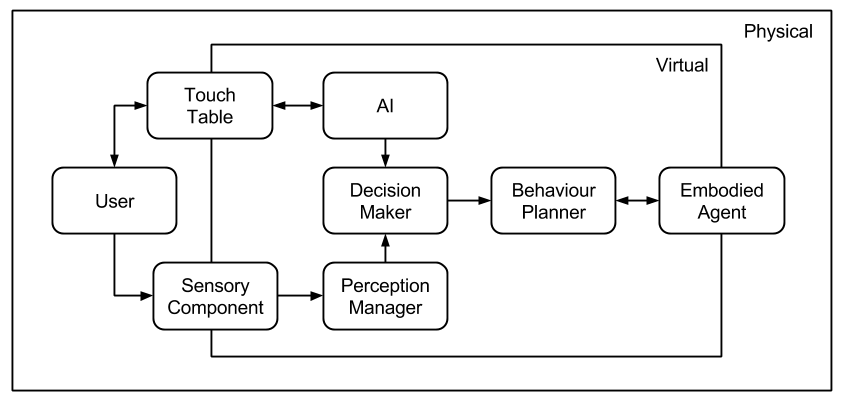
\includegraphics[width=1\textwidth]{./img/model}
  \caption{Structure of the social robot that plays \emph{Sueca}}
\label{fig:model}
\end{figure}

This model distinguishes physical components from virtual ones.
Some entities are not detailed on the scope of this project and are presented as both physical and virtual components.
The human players, Users, will play with physical cards on top of a Touch Table.
Every game action is detected and communicated to both the \gls{ai} module and the Perception Manager.
The Perception Manager receives information from all the Sensory Components.
The \gls{ai} module includes all the reasoning about the game and decides the robot's next move.
However, the robot's actions also involve social behaviours and these are managed by the Decision Maker.
The Decision Maker balances the \gls{ai} decision, sensory components and table events that represent states of the game.
It aims to produce appropriate behaviours depending on the situation.
For instance, being the last player of a trick and taking the two highest cards of a suit by playing a trump card is an exciting move and should produce an equally exciting reaction on the robot.
Lastly, the Behaviour Planner builds a suitable plan to execute the chosen high-level behaviour while considering the state of the embodied agent.

The architecture that will instantiate the model described above is partially decided.
The virtual layer will be mainly covered by Thalamus framework, which enables the communication between the mentioned entities \cite{Ribeiro}.
The chosen Behaviour Planner is Skene \cite{Ribeiroa}.
The \gls{ai} module will be processed offline with the algorithms described in Section~\ref{sec:sueca_solution}.
The embodied agent will initially be \gls{emys} due to its expressiveness, although other robots will be considered, depending on the users' preferences.
Finally, the undecided components are the sensory inputs.
Pereira et. al. have shown the importance of collecting data from user studies.
These components will be settled further, after some field research with \emph{Sueca} players.










\section{Evaluation Methodology} \label{sec:evaluation}

The correctness and benefits of the proposed work must be evaluated.
Firstly, it will be settled a proper user study of elderly playing \emph{Sueca} with \gls{emys}.
Each group will play a tournament with two different versions of the embodied agent:
\begin{itemize}
\item An agent that plays the game with few or nonexistent social behaviours;
\item An agent that plays the game and reacts according to the game state with verbal and nonverbal cues.
\end{itemize}
After the tournament, each person will answer a questionnaire in order to evaluate the individual experience and feelings during the game.
On one hand, the questionnaire will compare the experience with a robot versus the traditional card game.
On the other hand, it will compare the two versions of the agent and understand how the presence of each version of the robot was perceived.

Secondly, finding a group of elderly to do a user study is not so simple.
Considering such problems, the evaluation of the artificial player will not be made with aged people.
Due to the college environment where this work takes place, the university community will attend to tournaments in order to do this evaluation.
The performance of the the artificial player will be measured by the percentage of winning games.
\section{Conclusion} \label{sec:conclusion}

The pertinence of this work has been demonstrated considering the related work presented.
The state of the art robots for elderly is focused on service robots to guide them in their daily tasks.
Considering the companion type robots for aged people, existing technology is focused on therapy especially for the disabled.
On the other hand, the proposed robot aims to interact with elderly in a specific scenario for an entertainment and stimulating activity.
The \emph{Sueca} player will be based on Monte Carlo methods that are currently being successfully used on similar card games.


\nocite{*}
\bibliographystyle{splncs03}
\bibliography{references}



\end{document}
